\chapter{Bifurcation Theory and Physics of Confinement}\label{chapter:physics_bifurcation}

\section{Bifurcation Theory}\label{sec:bif_theory}
The aforementioned transitions show clear evidence of bifurcations in the plasma system.
%A defining feature of L--H transitions is that they can occur very suddenly (the so-called sharp transition), which is characteristic of fold bifurcation behavior.
Mathematically, a bifurcation is defined to be a topological or qualitative change in a system when a small and smooth change of a parameter is made.
A simple example for a fold bifurcation is the following, with $a$ representing the parameter:
\begin{equation} % Simplest fold bifurcation
	\frac{\text{d}x}{\text{d}t} \,=\, \dot{x} \,=\, a \,+\, x^2.
	\label{eq:simple_fold}
\end{equation}
This equation can behave in one of three manners:
If $a > 0$, there are no real points of equilibrium, also known as steady-state solutions.
For $a = 0$, there is one equilibrium point at $x = 0$, and two for $a < 0$, at $x = \pm\sqrt{-a}$.
Varying $a$ from some positive real number to some negative number, the fundamental behavior of the solutions changes drastically at $a = 0$ with the sudden appearance of a steady-state solution.
Equation~\ref{eq:simple_fold} is the simplest known form of a fold bifurcation, also known as the saddle-node bifurcation.
The simplest form for any dynamical system is known as the topological norm form.
A parameter plot of $x$ versus $a$ in Fig.~\ref{fig:simple_fold} illustrates this, with the green and red curves representing the stable and unstable steady-state solutions, respectively.

%{{{ Two figures for simple bifurcations (co-dimension 1 and 2)
\TwoFig{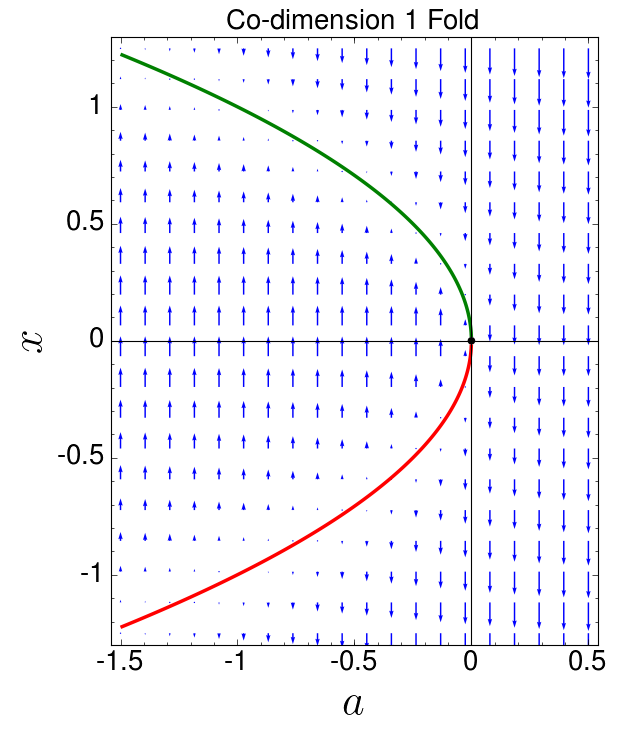
\includegraphics[width=\textwidth]{../Graphics/Bif_Graphs/Simple_fold.png}}
	{Plot of parameter space for $\dot{x} = a + x^2$ (Eq.~\ref{eq:simple_fold}), with the co-dimension 1 bifurcation occurring at $a = 0$. %
	For $a < 0$, the system has two steady-state solutions; the green is stable, while the red is unstable.
	For $a > 0$, there is no steady-state solution.}
	{fig:simple_fold}
	{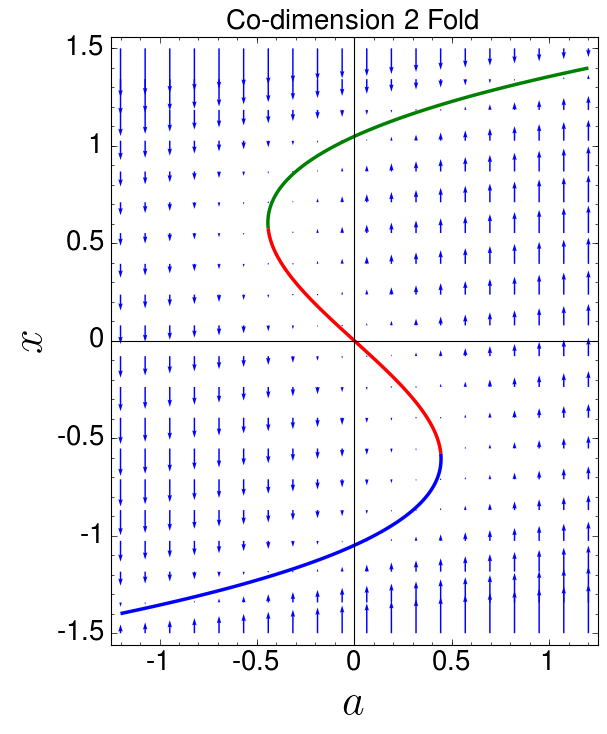
\includegraphics[width=\textwidth]{../Graphics/Bif_Graphs/co-2_fold.png}}
	{Plot of parameter space for $\dot{x} = -(a + x - x^3)$ (Eq.~\ref{eq:sharp_bif}). %
	This system showcases two fold bifurcations (each of co-dimension 1), at the turning points $a_{\pm\text{crit}}$, with two stable regions, in green and blue. %
	The red region is an intermediate that is unstable.}
	{fig:co-2_fold}
%}}}

The co-dimension of a system refers to the lowest number of parameters required to produce the topological norm form.
Put differently, it is the number of parameters that must be varied for the bifurcation to occur.
In the case of Eq.~\ref{eq:simple_fold}, there is only a single parameter, and is thus referred to as a co-dimension 1 bifurcation \cite{weymiens_bifurcation_2014}.

\subsection{Sharp and Smooth Transition Bifurcations}
%{{{ Two figures for zeros of the co-dimension 2 bifurcation
\TwoFigOneCap{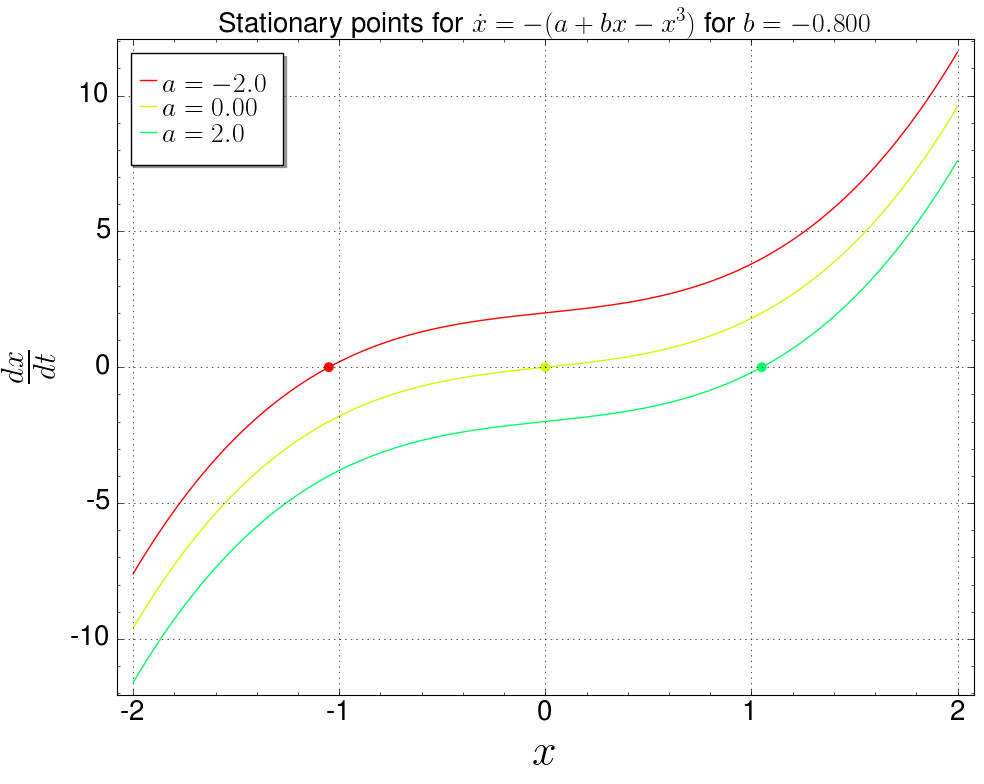
\includegraphics[width=\textwidth]{../Graphics/Bif_Graphs/stationary_b-0_8.png}}
	{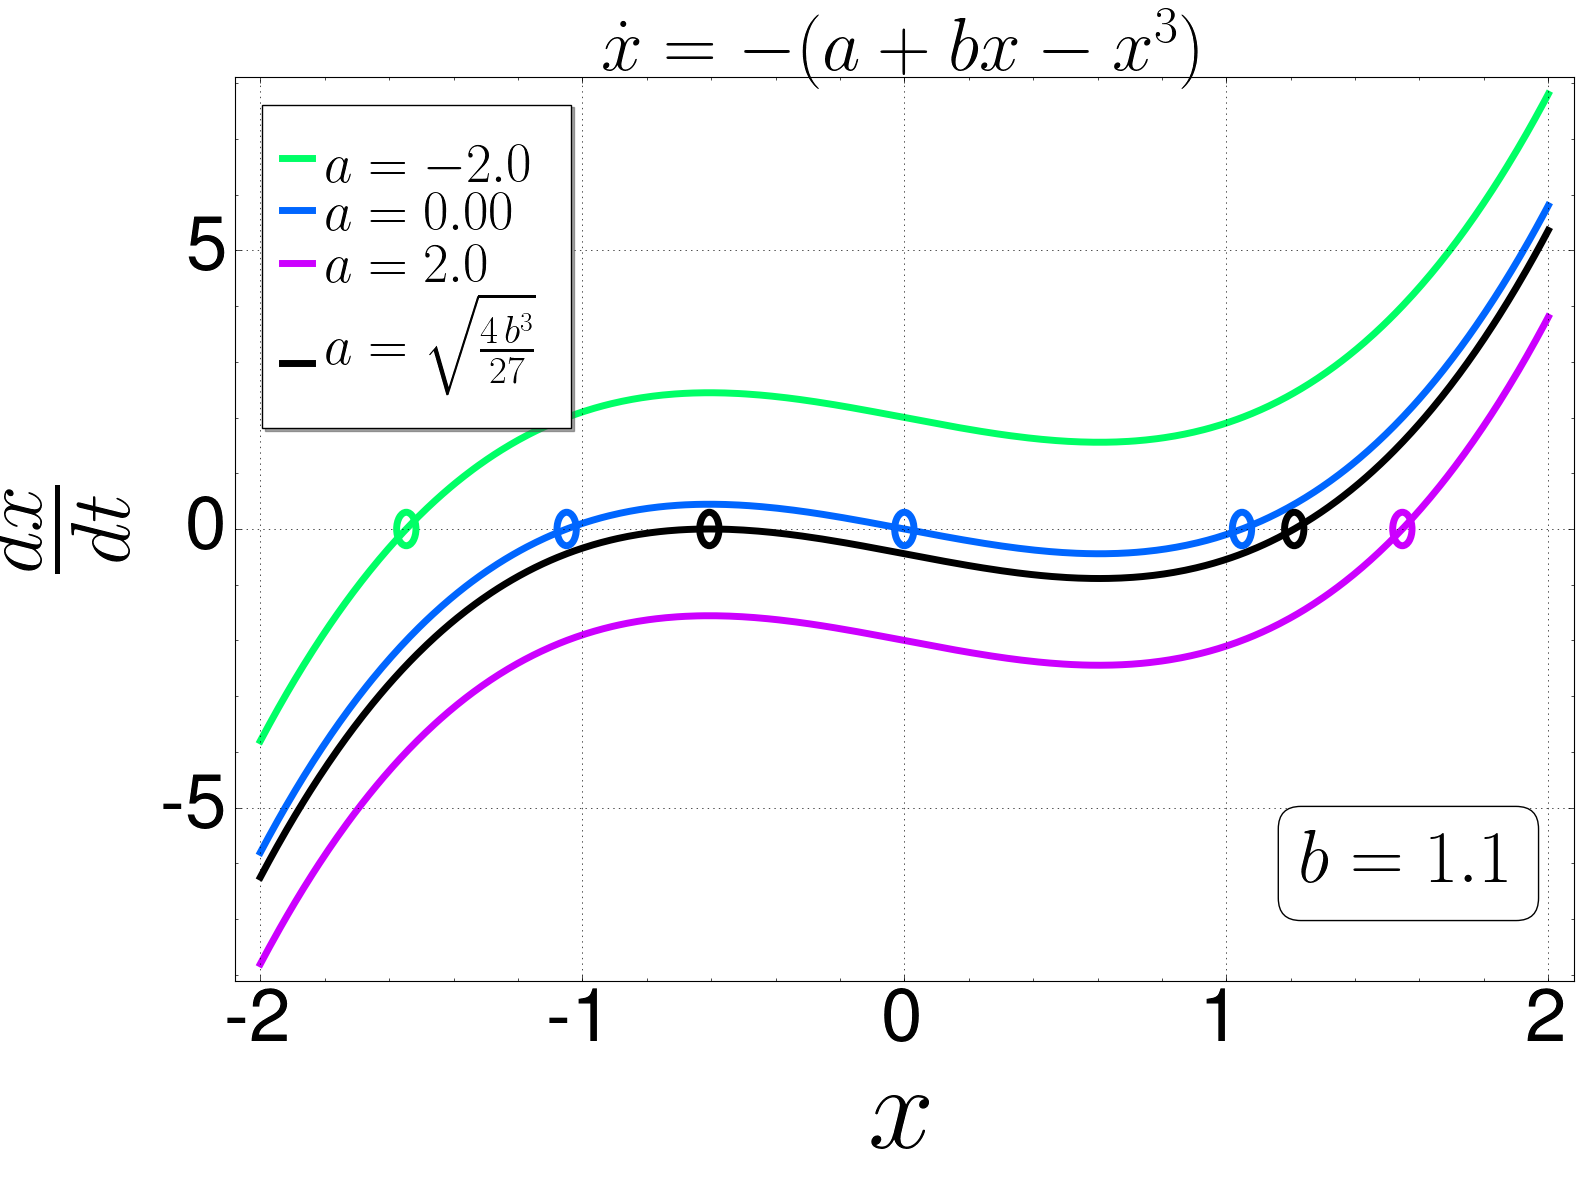
\includegraphics[width=\textwidth]{../Graphics/Bif_Graphs/stationary_b_1_1.png}}
	{Phase plots for Eq.~\ref{eq:sharp_bif}, with different values of $a$ within each plot. %
	There is a variance in the number of zeros based on the values of $a$ in the right plot, while there is strictly one zero for all values of $a$ in the left plot. %
	When there is multiple roots, the middle zero is always unstable.}
	{fig:stationaries_b}
%}}}

The dynamic behavior of the L--H transition correspond very closely to a few certain bifurcations.
Sharp and smooth transitions are features of the cusp bifurcation.
The topological norm form of this behavior is
\begin{equation}
	\dot{x} \,=\, -(a \,+\, bx \,-\, x^3)~.
	\label{eq:sharp_bif}
\end{equation}
Figure~\ref{fig:co-2_fold} is a plot of the parameter space, indicating the stable and unstable steady-state solutions.
This cusp bifurcation can also be regarded as two co-dimension 1 folds, if one views the positive and negative $x$-domains as separate co-dimension 1 bifurcations.
The distinction between sharp and smooth transitions in this co-dimension 2 bifurcation is solely based on the $b$ parameter, shown in the plots of Figure~\ref{fig:Bif_hysteresis}.
As $b$ approaches zero from some positive value, the size of the hysteresis shrinks, with it vanishing at $b = 0$, in which the smooth transition occurs.

%{{{ Two figures for co-dimension 2 bifurcation, with surface plot
\TwoFigOneCap{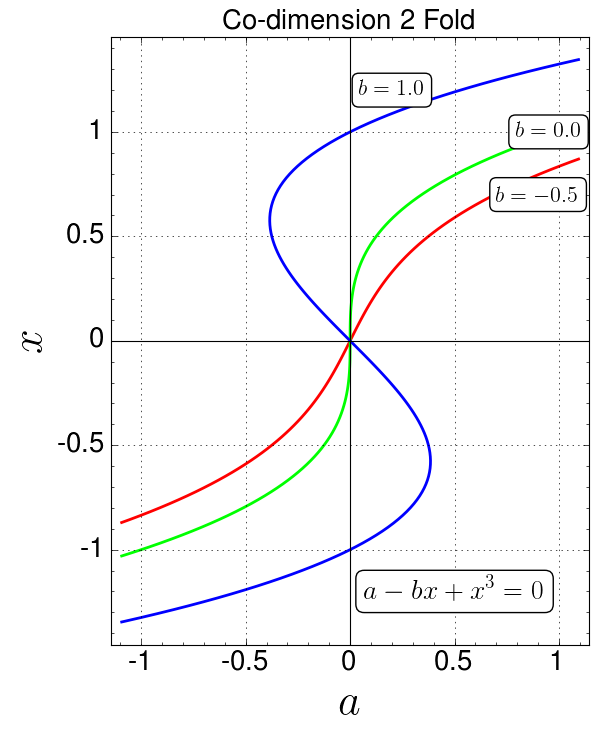
\includegraphics[width=\textwidth]{../Graphics/Bif_Graphs/co-2_fold_b_var.png}}
	{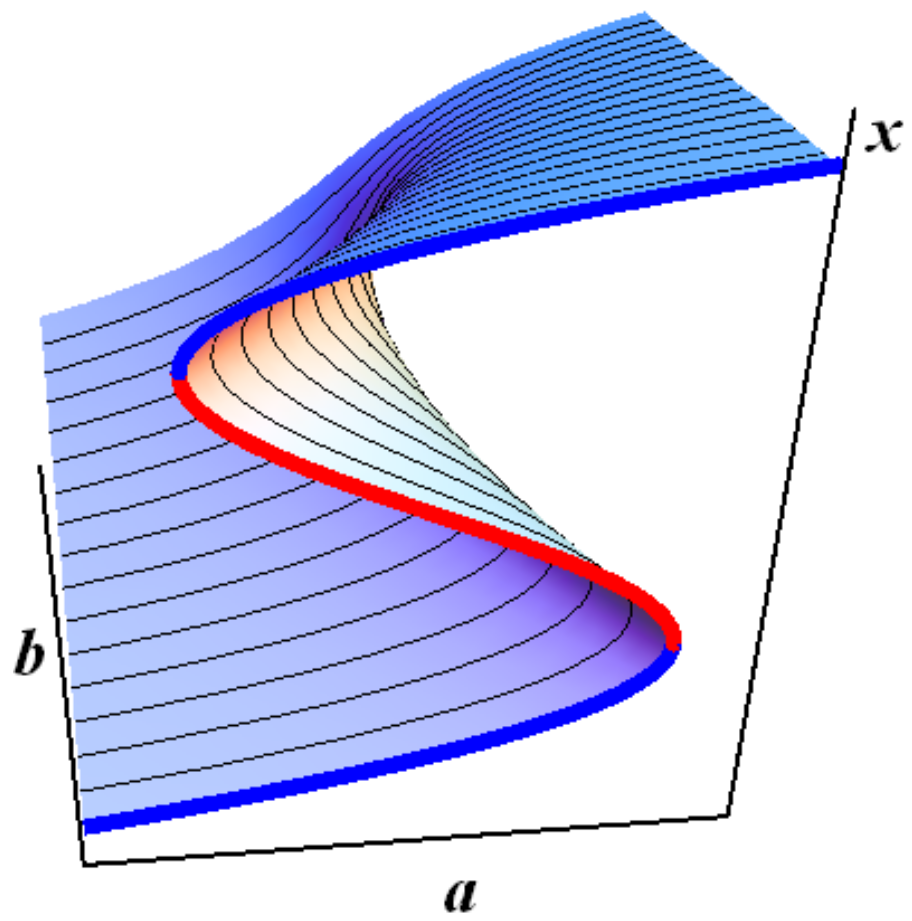
\includegraphics[width=\textwidth]{../Graphics/Bif_Graphs/Bif_3D.png}}
	{These plots show the mentioned co-dimension 2 cusp bifurcation, composed of two co-dimension 1 fold bifurcations, as described by Equation~\ref{eq:sharp_bif}.
	The plot on the left shows cross-sections for different $b$ values, with the sharp-smooth boundary occurring at $b = 0$.
	The plot on the right is the surface plot of this same model \cite{weymiens_bifurcation_2014}.}
	{fig:Bif_hysteresis}
%}}}

\subsection{Oscillatory Transition Bifurcation}
The third type of transition dynamics in tokamak plasmas is oscillatory, in which the system rapidly oscillates between the two different modes \cite{ryter_survey_2013, zohm_mhd_1995}.
This phenomenon is referred to by various names, including dithering, I--mode, predator--prey oscillations, and limit cycle oscillations.
It is the most enigmatic of the three discussed, as the least is known about it, and requires a more-complex model than Eq.~\ref{eq:sharp_bif}.

The Hopf, also known as a Poincar\'e-Andronov-Hopf, bifurcation is another co-dimension 1 bifurcation which can describe the oscillatory transition.
It occurs when a periodic solution or limit cycle that surrounds an equilibrium point arises or disappears, when varying the parameter.
Specifically, it occurs where the real part of complex conjugated eigenvalues vanish \cite{munoz-alicea_introduction_2011}.
%{{{ Hopf Bif example and sub/super critical explanation
%When a stable limit cycle encloses an unstable equilibrium point, it is denoted as supercritical.
%For an unstable limit cycle enclosing a stable equilibrium point, it is denoted subcritical.
%The norm form of the bifurcation is as follows,
%\begin{align} % Hopf bifurcation
%	\dot{x} \,=\, x\left((\lambda + i) + b|x|^2\right)~,
%	\label{eq:hopf_bif}
%\end{align}
%with $x$ and $b$ as complex-valued.
%Consider the following polar system, with $a$ as the parameter
%\begin{subequations}
%\begin{align} % Hopf example
%	\dot{r} \,&=\, a r - r^3~, \\
%	\dot{\theta} \,&=\, -1
%\end{align}
%\end{subequations}
%}}}

\subsection{Co-dimension 3 Bifurcation}
\begin{figure}[tb] % Co-dimension 3 bifurcation cross-section
\begin{minipage}{0.49\linewidth}
	\centering
	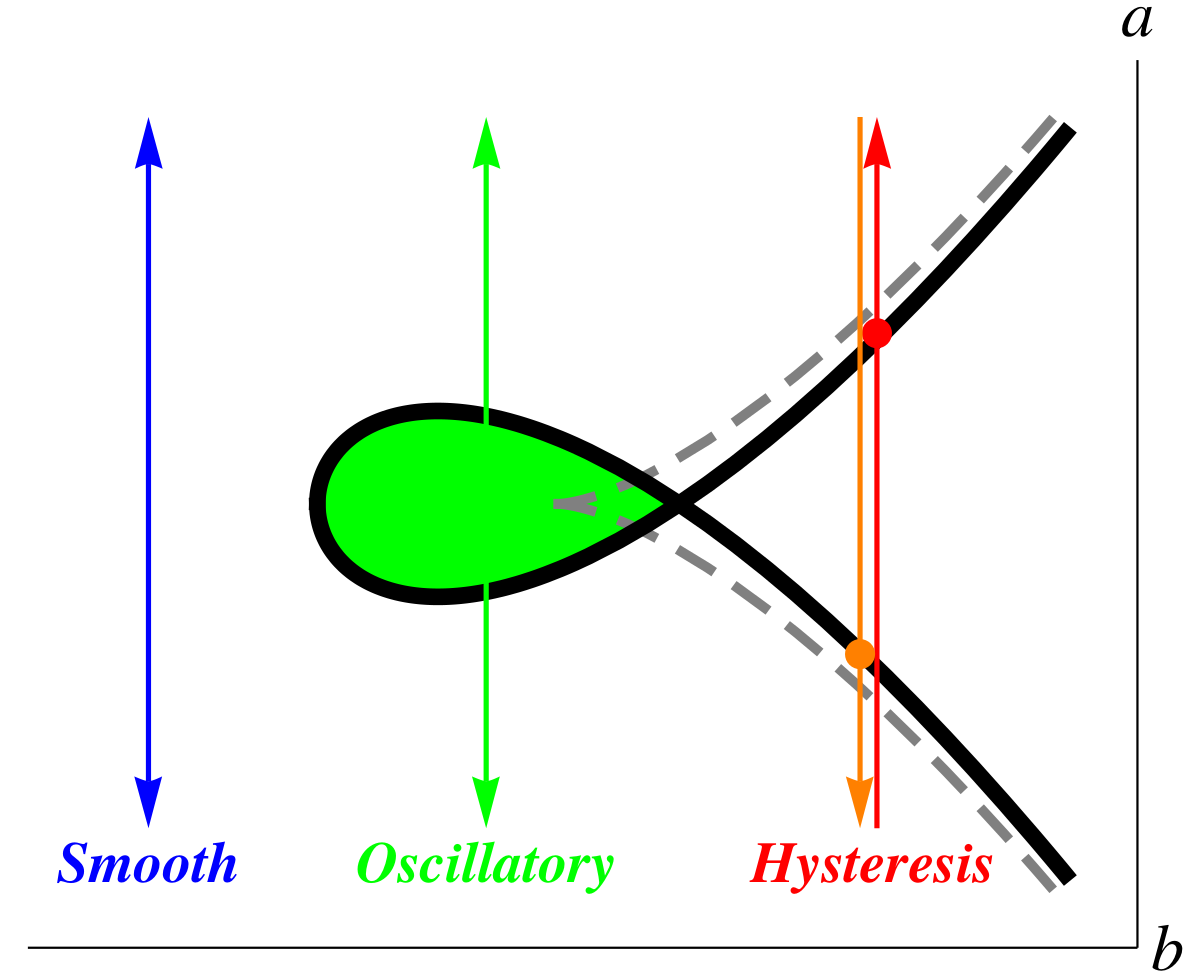
\includegraphics[width=0.9\textwidth]{../Graphics/Bif_Graphs/3_transitions_single_simple.png}
\end{minipage}
\hfill
\begin{minipage}{0.49\linewidth}
	\caption{A parameter plot of the FitzHugh-Nagumo model (Equations \ref{eq:FitzHugh-Nagumo}), a co-dimension 3 bifurcation with the black line indicating the fold bifurcation.
	This model is the one under consideration for accurately describing the L--H transition in tokamak plasmas, with the $b$ parameter dictating the type of transition.
	This $b$ parameter is akin to the density at the edge \cite{weymiens_bifurcation_2014}.}
	\label{fig:co-3}
\end{minipage}
\end{figure}

In order to accurately model to our current knowledge, the oscillatory transition must be incorporated with the sharp and smooth transitions.
Work by Weymiens \cite{weymiens_bifurcation_2014} proves that a ``co-dimension 3 bifurcation robustly connects the three types of transition behavior'' and investigates using the FitzHugh-Nagumo model.
\begin{subequations}
\begin{align} % FitzHugh-Nagumo model
	\dot{x} \,&=\, a - bx - x^3 + cy~, \\
	\dot{y} \,&=\, -y - x~.
\end{align}
	\label{eq:FitzHugh-Nagumo}
\end{subequations}
This couples the cusp bifurcation to a damped variable, with the coupling parameter $c$.
For as long as $c$ is below some critical value, only the cusp bifurcation will be present; a large enough value gives rise to the oscillatory transition.

All three bifurcations are shown in parameter space in the right plot of Fig.~\ref{fig:co-3}, with the value of the $b$ parameter dictating the type.

\subsection{Hysteresis}\label{ssec:hysteresis}
Hysteresis is a characteristic of any system which the current state of the system depends on its history.
In physics, the most common example given is that of an external magnetic field applied to a ferromagnetic material.
When the field is removed, the material will retain some of alignment of magnetic domains, and is considered magnetized.
Of course, this property is present in many other areas of study.

As mentioned previously, the L--H transition can be characterized with hysteresis.
The threshold power for the H--L transition can be significantly lower than that of the L--H transition, leading to a region in which there is a non-unique solution to the plasma state.
This requires two separate fold bifurcations each to govern the L--H and H--L transitions separately, which, in turn, requires two types of bifurcation parameters.
The first dictates hysteresis being present in the system; varying this allows for the disappearance of hysteresis when the aforementioned two fold bifurcations merge into a cusp bifurcation.
Varying the second parameter can cause the two stable solutions to be replaced by with unstable solutions, in which the system will oscillate between the solutions.
In the FitzHugh-Nagumo model (Eq.~\ref{eq:FitzHugh-Nagumo}), these are represented by $b$ and $c$, respectively.


\section{Mechanics}\label{sec:mechanics}
Physically, the L--H transition is a bifurcation in the turbulent transport at the edge of the tokamak.
The prevailing hypothesis for the overarching mechanism for H--mode that can be directly manipulated is that high auxiliary power develops strong sheared plasma flow and suppresses transport \cite{freidberg_plasma_2007}.

\subsection{Turbulence and Flow Shear Suppression}\label{ssec:turbulence_sheared}
Turbulence is primarily driven by the gradients of the temperature and density, which increase under higher heating.
Drift waves are considered to be the only type of turbulence that pushes radial particle flux; therefore, it dictates the severity of turbulence and linked transport at the edge of the plasma.
Particular well-known instabilities can be coupled to the drift-wave turbulence, such as the drift resistant ballooning mode, among others \cite{scott_three-dimensional_1997}.
Therefore, a form for the turbulence level will be restricted to one that adheres to the drift wave.

The turbulence $\mathcal{E}$ evolves as the following, in the absence of shear in the plasma flow
\begin{align} % Turbulence ODE
	\frac{\partial\mathcal{E}}{\partial t} \,=\, \gamma_L\mathcal{E} - \alpha_\text{sat}\mathcal{E}^2~.
	\label{eq:turbulence_ode}
\end{align}
This is the result from assuming the particle diffusivity increases linearly with the level of turbulence up to some maximum \cite{diamond_dynamics_1995}.
The first term on the right-hand side is a linear growth term, with $\gamma_L$ as the growth rate.
The second term is a nonlinear saturation term, with $\alpha_\text{sat}$ as the saturation rate.
The maximum turbulence is the ratio of the linear growth rate to the saturation rate.

It is now accepted that turbulent transport at the edge is particularly suppressed by shear in the flow of the $\mathbf{E}\times\mathbf{B}$ drift \cite{terry_suppression_2000}.
The shear stress dissociates smaller turbulent structures, with their energy and momenta transferred to larger flows.
This flow shear can be modeled as a ratio of the electromagnetic fields given by \cite{staps_backstepping_2017}
\begin{align} % Shear velocity
	\frac{\partial V_{\mathbf{E}\times\mathbf{B}}}{\partial x} \,=\,
		\frac{\partial}{\partial x} \left(\frac{E_r}{B}\right) \,\approx\,
		\frac{1}{B_\phi} \frac{\partial E_r}{\partial x}~.
	\label{eq:velocity_shear}
\end{align}
Both zonal and mean $\mathbf{E}\times\mathbf{B}$ flows are responsible for the drift-wave turbulence.
Zonal flows in particular are present in L--mode, in which the shear due to Reynolds stress comes from radial and poloidal perturbations \cite{diamond_zonal_2005}.
However, they disappear in H--mode, leaving only mean flows present.

The flow shear could reduce the growth rate of the turbulence \cite{diamond_self-regulating_1994}, which was coined the linear model.
The other possibility is that flow shear can increase the saturation mechanism, which is the nonlinear model \cite{hahm_rotation_1994}.
Each are implemented as some parameter that multiplies against their respective term in Equation~\ref{eq:turbulence_ode}.
For example, the nonlinear model would adjust it to the following
\begin{align} % Nonlinear Turbulence ODE
	\frac{\partial\mathcal{E}}{\partial t} \,=\, \gamma_L\mathcal{E} -
		\eta_\text{NL}\alpha_\text{sat}\mathcal{E}^2~, ~~~~ \eta_\text{NL} \,=\,
		1 + \tilde{\eta} \left|\frac{\partial V_{\mathbf{E}\times\mathbf{B}}}{\partial x}\right|^2.
	\label{eq:nonlinear_turbulence_ode}
\end{align}
Both forms were investigated by Weymiens, and the nonlinear model proved more robust to changes in plasma parameters \cite{weymiens_bifurcation_2014}.
Therefore, this nonlinear model will be used in this study.

In slab geometry, a radial electric field is proportional to $V_{\mathbf{E}\times\mathbf{B}}$, allowing us to substitute in $Z$, a form of the radial electric field that is normalized with the temperature $T$ and poloidal ion (Larmor) gyroradius $\rho_{\theta i}$.
The definition of $Z$ is shown as Eq.~\ref{eq:Z_and_rho_definitions} in Section \ref{ssec:E_r}.
This changes the coefficient of the nonlinear turbulence model $\eta_\text{NL}$ into
\begin{align} % New Saturation Coefficient
	\eta_\text{NL} \,=\, 1 +
		\tilde{\eta} \left|\frac{\partial V_{\mathbf{E}\times\mathbf{B}}}{\partial x}\right|^2
		\,=\, 1 + \eta\left|\frac{\partial Z}{\partial x}\right|^2~,
	\label{eq:saturation_normalization}
\end{align}
with $\eta$ including the normalization.

\subsection{Radial Electric Field}\label{ssec:E_r}
To generate a poloidal $\mathbf{E}\times\mathbf{B}$ flow with a mainly toroidal $\mathbf{B}$, an electric field must be generated.
A plethora of individual processes for the generation of such an electric field have been proposed, most of which can be viewed as separate contributions in a radial Poisson's law, with some that tend to reduce the field.
The radial electric field $E_r$ can be deduced from the radial force balance in steady-state for any plasma species $j$, as follows:
\begin{equation} % Lorentz Force Balance
	E_r \,=\, -\frac{1}{n_j e_j} \frac{\text{d} p_j}{\text{d} r} + V_{\theta j} B_\phi - V_{\phi j} B_\theta
	\label{eq:E_r}
\end{equation}
In the above, $e_j$ represents the charge of the $j$-th species, $n_j$ is the density, $p_j$ is the pressure, and $V_{\theta j}$ and $V_{\phi j}$ are the poloidal and toroidal velocities, respectively.
This grants changes in the radial electric field to be associated with changes in radial gradient of the pressure or either velocities \cite{connor_review_2000}.
Experimentally, each term can be measured separately; however, determining these values is difficult due to large possible error.

As alluded to in the previous section, a definition of the normalized radial electric field is needed.
The definition used is
\begin{align} % Z definition
	Z \,\equiv\, \frac{\rho_{\theta i} \, e \, E_r}{T_i}~, ~~~~
		\rho_{\theta i} \,\equiv\, \frac{m_i \, v_{T_i}}{e \, B_\theta}~,
		\label{eq:Z_and_rho_definitions}
\end{align}
with the ion mass $m_i$, the thermal ion velocity $v_{T_i}$, the elementary charge $e$, and the poloidal magnetic field $B_\theta$.

Rather than looking at an overall effect, an alternate method to determine the electric field is to look for the sources.
This means investigating the particle fluxes that go across the magnetic flux surfaces.
Any radial fluxes can be categorized as ambipolar or nonambipolar.
Ambipolar fluxes have an equal effect on electrons and all species of ions, resulting in no overall radial current.
Nonambipolar fluxes affect various charged particles differently, and thus create an electric field.
This resulting field creates a return current so that the divergence of the plasma current, on average, returns to zero.
The evolution of the field is determined by the sum of all possible radial currents, with $\Gamma_j^\text{k}$ referring to only nonambipolar fluxes of species $j$, since those are the ones to contribute to the field.
\begin{align} % Ambipolarity constraint
	\epsilon_0 \frac{\partial E_r}{\partial t} \,=\, -\sum J_r \,=\,
		\sum_\text{k} q_j\Gamma_j^\text{k} \label{eq:ambipolarity_constraint}
\end{align}

Kinetic and atomic processes contribute to the nonambipolar fluxes, in addition to fluid processes implied by the description.
These include ion orbit loss and charge exchange friction.
Details on the nonambipolar fluxes utilized in this investigation are described in depth in Section~\ref{sec:nonambipolar_fluxes}.

